%%% Preamble
\documentclass{report}

\usepackage[utf8]{inputenc}
\usepackage[T1]{fontenc}
\usepackage{fourier}
\usepackage[french]{babel}
\usepackage[protrusion=true,expansion=true]{microtype}	
\usepackage{amsmath,amsfonts,amsthm} % Math packages
\usepackage[pdftex]{graphicx}	
\usepackage{url}
\usepackage{pdfpages}
\usepackage{todonotes}
\usepackage[a4paper, body={16cm,26cm}]{geometry}
\usepackage{float}
\usepackage{framed}
\usepackage[toc,page]{appendix} 
\usepackage{multicol}
\usepackage{colortbl}
\usepackage{epstopdf}
\usepackage{adjustbox}

%%% Custom sectioning
\usepackage{sectsty}
\allsectionsfont{  \normalfont\scshape}
%\allsectionsfont{\centering \normalfont\scshape}

%%% Custom headers/footers (fancyhdr package)
\usepackage{fancyhdr}
\pagestyle{fancyplain}
\fancyhead{}								% No page header
\fancyfoot[L]{}							% Empty 
\fancyfoot[C]{}							% Empty
\fancyfoot[R]{\thepage}					% Pagenumbering
\renewcommand{\headrulewidth}{0pt}		% Remove header underlines
\renewcommand{\footrulewidth}{0pt}		% Remove footer underlines
\setlength{\headheight}{13.6pt}


%%% Define new commands
\newcommand{\horrule}[1]{\rule{\linewidth}{#1}} 	% Horizontal rule
\renewcommand{\bf}[1]{\textbf{#1}}
\renewcommand{\it}[1]{\textit{#1}}
\renewcommand{\sc}[1]{\textsc{#1}}
\newcommand{\bfit}[1]{\textbf{\textit{#1}}}
\newcommand{\appname}{GFaim}

\newcommand{\modification}[1]{\todo[inline]{#1}}
\newcommand{\modificationFigure}{\todototoc}
\renewcommand{\thesection}{\thepart .\arabic{section}}

\usepackage{tocloft}
\cftsetindents{chapter}{0em}{1em}
\cftsetindents{section}{1.5em}{2.5em}
\makeatletter
\def\l@figure{\@dottedtocline{1}{1.5em}{4em}}
\makeatother
\PassOptionsToPackage{colorlinks=true,linkcolor=darkgray}{hyperref}
\usepackage{bookmark}
\usepackage{cases}
\usepackage{color}
\usepackage{xcolor}
\usepackage{relsize}
\usepackage{caption}
\colorlet{shadecolor}{black!10}

\delimitershortfall-1sp
\newcommand\abs[1]{\left|#1\right|}


\usepackage{tikz, pgfplots}


%}}}
%{{{ --- pgfplots ---------------------

%{{{ Colors

% TolColors from http://www.r-bloggers.com/the-paul-tol-21-color-salute/
\definecolor{TolColor1}{HTML}{332288}   % dark purple
\definecolor{TolColor2}{HTML}{6699CC}   % dark blue
\definecolor{TolColor3}{HTML}{88CCEE}   % light blue
\definecolor{TolColor4}{HTML}{44AA99}   % light green
\definecolor{TolColor5}{HTML}{117733}   % dark green
\definecolor{TolColor6}{HTML}{999933}   % dark brown
\definecolor{TolColor7}{HTML}{DDCC77}   % light brown
\definecolor{TolColor8}{HTML}{661100}   % dark red
\definecolor{TolColor9}{HTML}{CC6677}   % light red
\definecolor{TolColor10}{HTML}{AA4466}  % light pink
\definecolor{TolColor11}{HTML}{882255}  % dark pink
\definecolor{TolColor12}{HTML}{AA4499}  % light purple

%}}}
%{{{ Color cycles

\pgfplotscreateplotcyclelist{mbarplot cycle}{%
  {draw=TolColor2, fill=TolColor2!70},
  {draw=TolColor7, fill=TolColor7!70},
  {draw=TolColor4, fill=TolColor4!70},
  {draw=TolColor11, fill=TolColor11!70},
  {draw=TolColor1, fill=TolColor1!70},
  {draw=TolColor8, fill=TolColor8!70},
  {draw=TolColor6, fill=TolColor6!70},
  {draw=TolColor9, fill=TolColor9!70},
  {draw=TolColor10, fill=TolColor10!70},
  {draw=TolColor12, fill=TolColor12!70},
  {draw=TolColor3, fill=TolColor3!70},
  {draw=TolColor5, fill=TolColor5!70},
}

\pgfplotscreateplotcyclelist{mlineplot cycle}{%
  {TolColor2, mark=*, mark size=1.5pt},
  {TolColor7, mark=square*, mark size=1.3pt},
  {TolColor4, mark=triangle*, mark size=1.5pt},
  {TolColor6, mark=diamond*, mark size=1.5pt},
}


\pgfplotsset{
  compat=1.9,
  mbaseplot/.style={
    legend style={
      draw=none,
      fill=none,
      cells={anchor=west},
    },
    x tick label style={
      font=\footnotesize
    },
    y tick label style={
      font=\footnotesize
    },
    legend style={
      font=\footnotesize
    },
    major grid style={
      dotted,
    },
    axis x line*=bottom,
  },
  mlineplot/.style={
    mbaseplot,
    xmajorgrids=true,
    ymajorgrids=true,
    major grid style={dotted},
    axis x line=bottom,
    axis y line=left,
    legend style={
      cells={anchor=west},
      draw=none
    },
    cycle list name=mlineplot cycle,
  },
  mbarplot base/.style={
    mbaseplot,
    bar width=6pt,
    axis y line*=none,
  },
  mbarplot/.style={
    mbarplot base,
    ybar,
    xmajorgrids=false,
    ymajorgrids=true,
    area legend,
    legend image code/.code={%
      \draw[#1] (0cm,-0.1cm) rectangle (0.15cm,0.1cm);
    },
    cycle list name=mbarplot cycle,
  },
  horizontal mbarplot/.style={
    mbarplot base,
    xmajorgrids=true,
    ymajorgrids=false,
    xbar stacked,
    area legend,
    legend image code/.code={%
      \draw[#1] (0cm,-0.1cm) rectangle (0.15cm,0.1cm);
    },
    cycle list name=mbarplot cycle,
  },
  disable thousands separator/.style={
    /pgf/number format/.cd,
      1000 sep={}
  },
}


\usepackage{colortbl}
\usepackage{array}
\usepackage{ragged2e}
\newcolumntype{P}[1]{>{\RaggedRight\hspace{0pt}}p{#1}}

%%  ========   IMPORTANT ========
%% Indiquer ici les parties que vous voulez compilez

%%% Begin document
\begin{document}

\includepdf[pages={1}]{title.pdf}

\listoftodos[Todo List]
\newpage
\tableofcontents
{%
\let\oldnumberline\numberline%
\renewcommand{\numberline}{\figurename~\oldnumberline}%
\renewcommand\listfigurename{Liste des figures}
\listoffigures%
}
{%
\let\oldnumberline\numberline%
\renewcommand{\numberline}{\tablename~\oldnumberline}%
\renewcommand\listtablename{Liste des tableaux}
\listoftables%
}

\newpage
\addcontentsline{toc}{part}{Introduction}
\chapter*{Introduction}
\section*{Présentation du contenu du rapport}

\appname~n'est pas qu'une simple application permettant à l'utilisateur de choisir un restaurant, c'est bien plus que cela. \appname, c'est la garantie de ne jamais sortir d'un restaurant le ventre vide, et de ne jamais y entrer sans savoir si l'attente sera plus longue que le temps dont nous disposons. En effet, qui n'est jamais sorti déçu d'un restaurant, sans avoir pu manger car le temps d'attente était bien trop long, ou bien les prix trop élevés ? Grâce à \appname, ce ne sera plus un souci !\\
Le but de cette application est d'offrir à l'utilisateur un moyen simple et intuitif de repérer tous les restaurants alentours, leur distance à pied, et même l'attente en temps réel. Mais de nombreuses autres fonctionnalités existent également : programmer des notifications pour être prévenu de l'affluence de son restaurant favori juste avant d'aller manger, visualiser tous les restaurants proches sur une carte, ou encore voir les avis d'autres utilisateurs sur tel ou tel point de restauration.\\
En réalisant cette application, notre objectif était simple : répondre au besoin grandissant d'utilisateurs souhaitant optimiser leur emploi du temps. En effet, dans un environnement où tout évolue rapidement et où le temps se fait précieux, il est impensable de devoir attendre une heure avant de pouvoir être servi. Cependant, dans le cadre de ce projet, nous nous arrêtons à l'aspect visuel de l'application, en ne réalisant que les interfaces.

\part{Analyse des besoins}
\setcounter{section}{0}

\section{Généralités}

Avant de commencer un projet de ce type, il est très important de se renseigner sur ce qu'attendent les futurs utilisateurs de notre application, afin de pouvoir guider notre conception et ainsi ne pas développer des fonctionnalités qui ne trouveraient pas leur public. De plus, nous ne souhaitons pas restreindre l'application au campus, et de ce fait le recueil des besoin doit aussi se faire sur d'autres campus, qui n'auraient pas la même disposition et donc auraient d'autres besoins. C’est dans cette optique que nous avons décidé de concevoir un questionnaire que nous pourrions envoyer au plus grand nombre, et ce dans toute la France.

\section{Conception du questionnaire}

Le questionnaire que nous avons conçu s'oriente vers deux axes principaux : identifier les informations qui pourraient intéresser les utilisateurs et les fonctionnalités qui pourraient leur plaire. \newline
Pour ce faire, nous avons préalablement déterminé un ensemble d'informations qui nous semblent pertinentes pour différents points de l'application. Par exemple, quels points de restauration prendre en compte, quels indicateurs afficher pour permettre aux utilisateurs de faire un choix parmi ces derniers. Pour ces questions, nous avons conçu des questions à choix restreints, c'est-à-dire que nous ne demandons pas simplement une réponse oui/non, mais une réponse qui apporte plus de nuance, comme une quantification de la fréquentation, ou des questions à choix multiples. Cela nous permet d'avoir des résultats pour lesquels on peut prendre en compte l'avis des utilisateurs qui ont des habitudes minoritaires par rapport aux autres. \newline
Quant aux propositions de fonctionnalités, nous avons choisi de proposer des idées et des les soumettre à l'avis des utilisateurs grâce à des réponses fermées, c'est-à-dire que nous voulons juste recueillir un avis de type intéressé/pas intéressé. Les utilisateurs ont souvent du mal à exprimer ce qu'ils souhaitent avoir exactement dans les programmes que l’on essaye de développer pour eux. Ainsi, en exprimant une idée sous cette forme, donc en demandant simplement son approbation, il peut facilement dire si l'idée lui semble pertinente ou non. Un champ libre en fin de questionnaire lui permet de proposer de nouvelles idées ou d'exprimer tout commentaire qu'il aurait envie de nous transmettre. \\

Une fois les questions identifiées, il a fallu soigner la rédaction et la présentation du questionnaire. En effet, un questionnaire de ce type est souvent rebutant du fait que les étudiants en reçoivent souvent et régulièrement à propos de différents projets. Ce questionnaire s'adressant plus particulièrement à des étudiants, nous avons donc essayé de le rendre attractif et convivial afin que les utilisateurs aient envie de le remplir du début à la fin, et ce en peu de temps.
Nous avons donc rédigé les questions une première fois, puis l'avons fait essayer à quelques camarades. Nous nous sommes vite rendus compte que ces dernières manquaient d'homogénéité et n'invitaient pas forcément l'utilisateur à répondre. Par exemple, les questions portant sur les fonctionnalités étaient de la forme \og{}Si nous vous proposions de faire ceci, seriez-vous intéressé ? Super/Bof\fg{}. Les testeurs qui ont lu le questionnaire sous cette forme ont trouvé que cette formulation était trop classique et qu'ils ne se sentaient pas forcément impliqués. Nous avons donc repensé toutes les questions afin de les rendre plus directes et surtout homogènes entre elles, notamment en utilisant le tutoiement. Les questions sur les fonctionnalités ressemblent maintenant à \og{}Faire ceci, ça t'intéresse ? Intéressé/Pas intéressé\fg{}. \newline
Au niveau de la forme, nous n'avons pas voulu utiliser le classique Google Form, qui est déjà trop utilisé autour de nous. De plus, Google Form renvoie l'image d’un questionnaire long et formel, ce qui n'était pas du tout en accord avec l'esprit de notre formulaire. Pour rappel, notre questionnaire se veut direct, convivial et accessible. Nous nous sommes finalement tournés vers Typeform, qui propose de réaliser des sondages multi-plateformes (gérant déjà le responsive pour les smartphones et tablettes), pour lequel on peut incorporer des icônes dans les réponses, permettant une lisibilité et accessibilité accrue. Avec son design moderne et ses outils de personnalisation, nous avons réussi à créer le questionnaire que nous avions imaginé. \\

Quelques retours utilisateurs sur notre questionnaire final :\\
\begin{description}
    \item \og{}Pas mal le formulaire\fg{}
    \item \og{}Superbe formulaire !\fg{}
    \item \og{}Excellent questionnaire avec un bon humour\fg{}
    \item \og{}Niveau approche des étudiants c’est super\fg{}
\end{description}

\begin{figure}[H]
    \label{fig-qcm-question}
    \noindent\makebox[\textwidth]{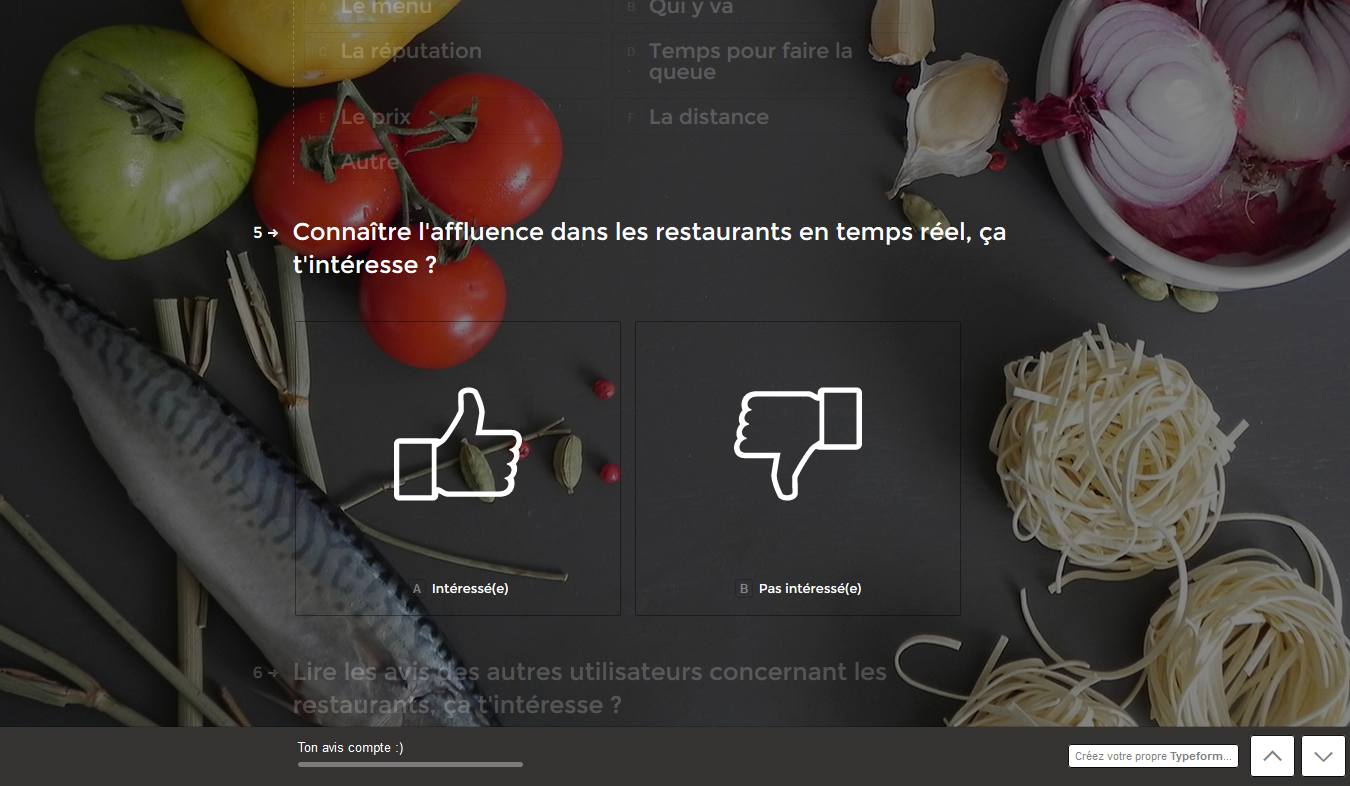
\includegraphics[width=10cm]{figures/qcm_question.png}}
    \caption{Capture d'écran d'une question du questionnaire}
\end{figure}

\section{Obtention et analyse des résultats}

Afin de réaliser une analyse multi-sites des besoins des potentiels utilisateurs de l'application, le questionnaire a été diffusé au sein de plusieurs campus de France, permettant ainsi d'obtenir des réponses de différentes régions. En effet, il est intéressant de combiner les besoins de différents profils d'utilisateurs, qui partagent tout de même une problématique commune. Ainsi, des réponses ont majoritairement été obtenues depuis les régions Auvergne, Bretagne, Centre et Rhône-Alpes. \\


\begin{figure}[H]
    \label{fig-carte-reponses}
    \noindent\makebox[\textwidth]{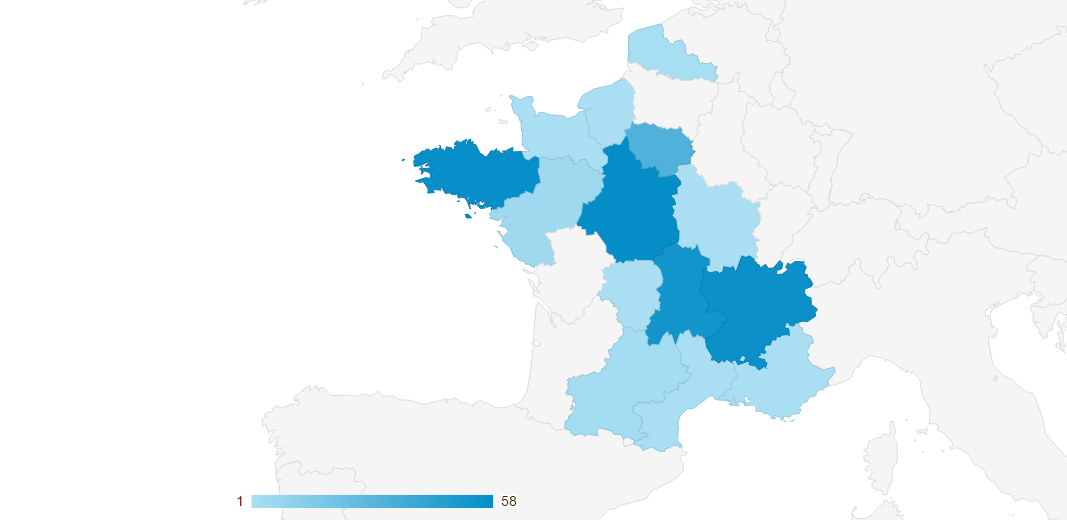
\includegraphics[width=10cm]{figures/carte_reponses.png}}
    \caption{Carte montrant la densité de réponses par régions}
\end{figure}

\begin{figure}[H]
    \label{fig-histo-reponses}
    \noindent\makebox[\textwidth]{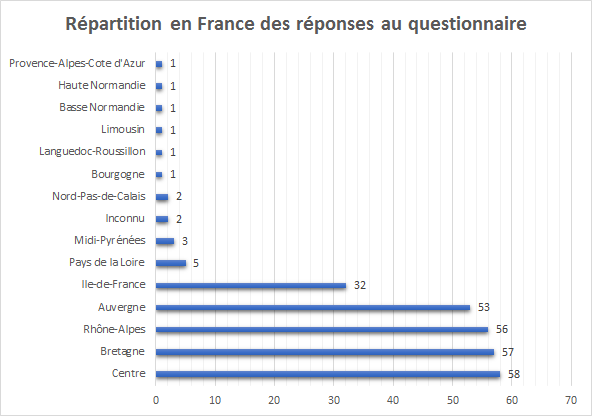
\includegraphics[width=10cm]{figures/histo_reponses.png}}
    \caption{Histogramme donnant le nombre de réponses par région}
\end{figure}

Grâce à cette diffusion inter-campus du questionnaire, 311 réponses ont été collectées. Certains internautes masquant leur position géographique lors de leur navigation, une légère différence est à relever entre le nombre de réponses total apparaissant sur le questionnaire et sur les graphiques de répartition géographique. L'ensemble des questions et des réponses associées sont disponibles en annexe. \\

L'échantillon visé étant une population étudiante, 91\% des répondants ont déclaré posséder un smartphone, confortant ainsi l'idée de développer une application mobile. En effet, 80\% des répondants ont également déclaré être intéressés par une application smartphone permettant de connaître les différents points de restauration autour de leur campus. Ce pourcentage est suffisamment significatif pour s'intéresser dans un second temps aux habitudes et aux besoins des étudiants. \\

Ainsi, au cours d'une semaine type, 68\% des répondants mangent souvent voir tout le temps dans un restaurant universitaire. Cependant, 18\% des étudiants interrogés mangent très peu voir jamais dans un restaurant universitaire. En effet, 35\% des étudiants déjeunent parfois dans un restaurant/snack situé en dehors du campus, tandis que 20\% des étudiants mangent de temps en temps un repas acheté au supermarché. Cette hétérogénéité des réponses illustre bien les différentes habitudes des étudiants au sein des différents campus universitaires. Ainsi, il est important d'indiquer dans notre application non seulement les restaurants universitaires, mais également les différentes alternatives, afin de répondre aux besoins de chacun. \\

Afin de déterminer quelles sont les informations à mettre en avant dans notre application, nous pouvons nous intéresser aux différents critères identifiés comme importants par les étudiants ayant répondu au questionnaire. Ainsi, 82\% des répondants considèrent le prix comme étant un critère important lorsqu'ils recherchent un endroit pour manger. 66\% des étudiants considèrent également la distance et le temps d'attente comme étant important, tandis que la réputation est un critère important pour seulement 12\% des répondants. De fait, notre application devra mettre en avant ces trois informations (prix, distance et temps d'attente) jugées comme critiques pour effectuer un choix. Ces données devront donc être visibles dès l'affichage réduit des lieux de restauration, les autres informations jugées comme étant moins importantes pouvant alors être visibles lors d’un affichage détaillé. \\

De même, 87\% des étudiants ayant répondu au questionnaire ont déclaré être intéressés pour connaître en temps réelle l'affluence des lieux de restauration. Ce pourcentage fortement significatif concorde avec la déclaration de l'importance du critère du temps d'attente pour choisir un lieu de restauration. Cette donnée étant particulièrement importante, il est nécessaire d'indiquer des valeurs s'approchant au mieux de la situation réelle. Pour cela, une interface pour restaurateurs est à prévoir dans notre application, afin de permettre à ces derniers de renseigner à intervalle régulier l’affluence de leur établissement. \\

Parmi les répondants au questionnaire, 77\% sont également intéressés par les avis des autres utilisateurs de l'application, sans pour autant rechercher un établissement présentant une haute réputation, cherchant ainsi les compromis. Nous pouvons donc prévoir un système d’évaluation des lieux de restauration par les utilisateurs de l'application, en demandant toutefois une notation numérique ainsi qu’une appréciation textuelle. Cela permettra de proposer dans un premier temps une notation moyenne. Dans un second temps, l'utilisateur aura la possibilité d'afficher l’ensemble des évaluations des utilisateurs, répondant ainsi au besoin exprimé à travers cette question. \\

A contrario, seulement 55\% des répondants sont intéressés par des informations diététiques sur les lieux de restauration et 45\% des étudiants ayant répondu sont intéressés par les avertissements et informations liés aux régimes particuliers. S'agissant de données importantes pour une minorité d'utilisateurs, ces informations pourront être paramétrées dans l'application afin d'activer leur affichage. \\

Concernant les fonctionnalités liées à la dimension sociale, celles-ci ne seront pas mises en avant dans l'application. En effet, 67\% des répondants présentent un intérêt pour la possibilité de convenir de rendez-vous avec leurs amis, tandis que seulement 32\% des étudiants souhaitent connaître les repas de leurs amis. Or, de nombreux outils existant permettant déjà de convenir d'un rendez-vous entre amis. Cette possibilité recueille en effet un bon pourcentage d'intérêt. Cependant, nombre de réactions négatives ont également été reçues quant à cette fonctionnalité. Ainsi, notre application ne comportera pas cette dimension sociale, afin de ne pas contraindre les utilisateurs sur le moyen de communication. \\

Le questionnaire comportait également un champ libre, permettant ainsi aux répondants de s'exprimer librement sur leurs besoins. Globalement, le concept de l’application a été bien accueilli, les étudiants émettant parfois leur souhait de voir l'application se réaliser afin de pouvoir l’utiliser par la suite. Ainsi, ce questionnaire nous a permis d'évaluer les différents besoins des étudiants à travers plusieurs campus qui présentent une même problématique, à savoir comment déterminer le lieu de restauration. Les informations à mettre en avant ont ainsi été déterminées, tandis que le bien fondé de l'application a été validé à travers ce questionnaire et son analyse. \\


\part{Analyse de l'existant}
\setcounter{section}{0}

\section{Applications existantes}

Aujourd'hui, il existe de nombreuses applications pour la recherche de restaurants : Yelp, Foursquare, Zomato, TripAdvisor et CROUS Mobile. Chaque application a sa propre particularité. \\

\bf{Yelp} est un site où sont répertoriés tout les avis des commerces locaux (alimentation, restaurant, shopping). Ce site est principalement actif dans les grandes villes.

\begin{figure}[H]
    \label{fig-yelp}
    \noindent\makebox[\textwidth]{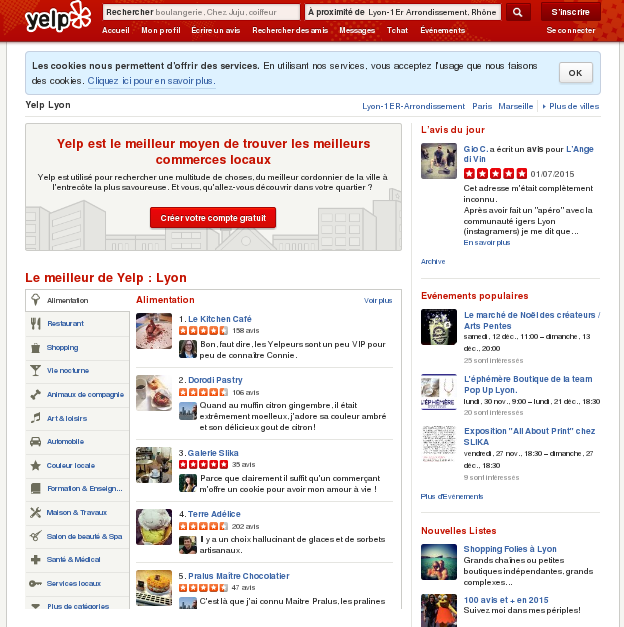
\includegraphics[width=10cm]{figures/yelp.png}}
    \caption{Capture d'écran de l'application Yelp}
\end{figure}

\bf{Foursquare} est un média social qui grâce à la géolocalisation permet à l'utilisateur de lui indiquer où il se trouve des lieux de sorties (restaurants, cafés, magasins).

\begin{figure}[H]
    \label{fig-foursquare}
    \noindent\makebox[\textwidth]{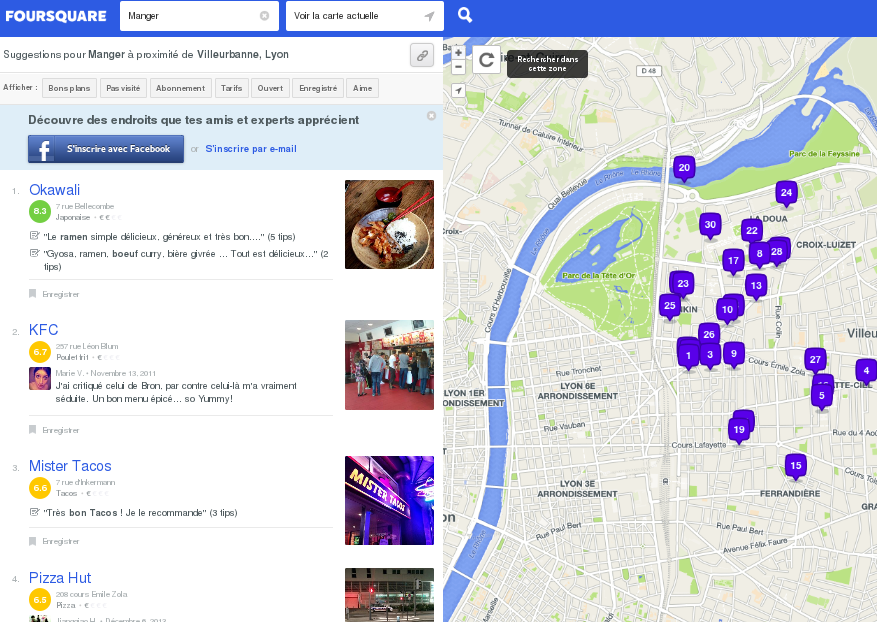
\includegraphics[width=10cm]{figures/foursquare.png}}
    \caption{Capture d'écran de l'application Foursquare}
\end{figure}

\bf{Zomato} est un annuaire des restaurants permettant de rechercher des informations sur les restaurants du monde entier (avis, photos). Il fonctionne sous la forme d'un réseau social où les utilisateurs publient des commentaires et des photos sur les restaurants et cela passe dans un fil d'actualité.

\begin{figure}[H]
    \label{fig-zomato}
    \noindent\makebox[\textwidth]{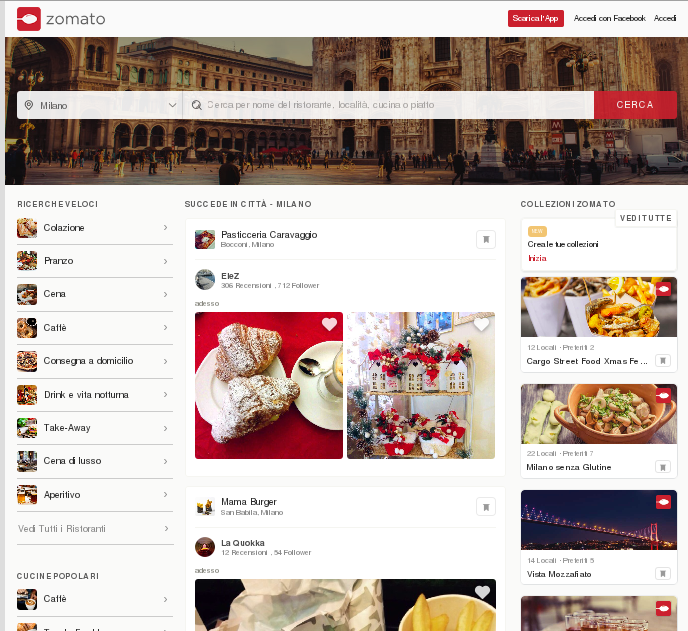
\includegraphics[width=10cm]{figures/zomato.png}}
    \caption{Capture d'écran de l'application Zomato}
\end{figure}

\bf{TripAdvisor} est un site web qui offre des avis et des conseils touristique de consommateur (hôtels, restaurants, villes et régions, lieux de loisirs) et fournit également des outils de réservation de logements et de billets d'avion comparant des centaines de sites web afin de trouver les meilleurs prix.

\begin{figure}[H]
    \label{fig-trip-advisor}
    \noindent\makebox[\textwidth]{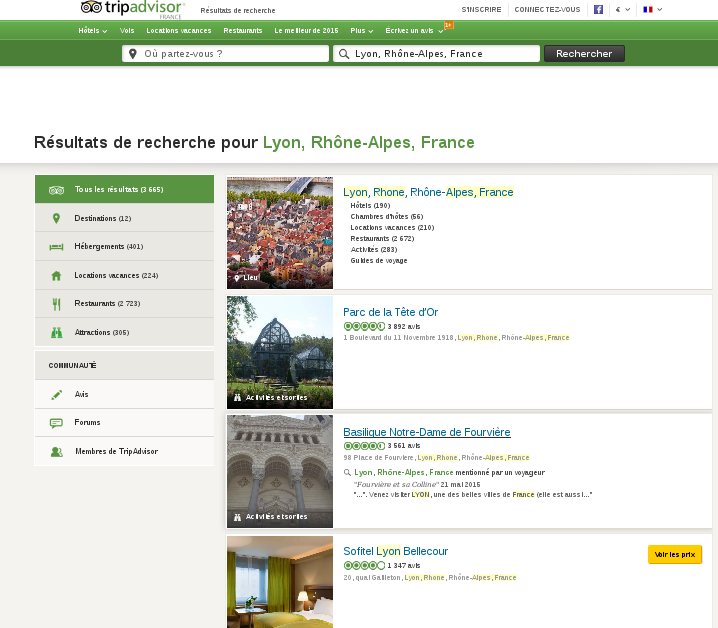
\includegraphics[width=10cm]{figures/trip_advisor.png}}
    \caption{Capture d'écran de l'application TripAdvisor}
\end{figure}

\bf{CROUS Mobile} est une application pour smartphone qui permet de retrouver toutes les informations du Crous (Restos U, logement, activités culturelles, services sociaux…).

\begin{figure}[H]
    \label{fig-crous-mobile}
    \noindent\makebox[\textwidth]{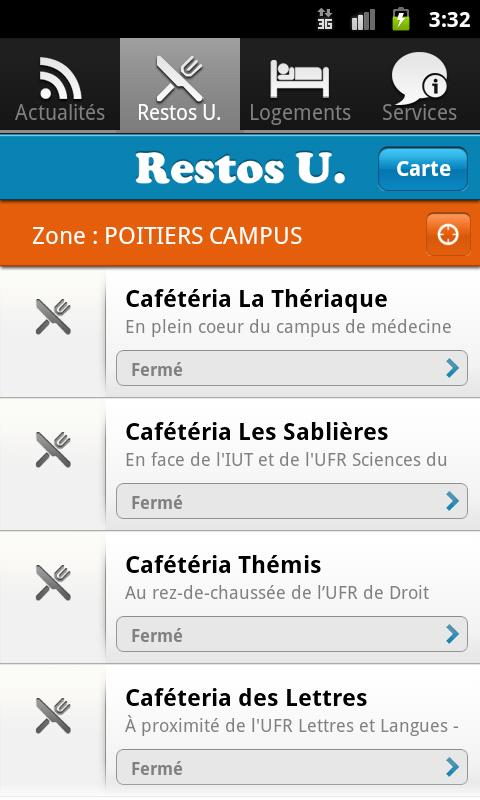
\includegraphics[width=6cm]{figures/crous_mobile.jpg}}
    \caption{Capture d'écran de l'application CROUS Mobile}
\end{figure}

\section{Conclusion}

Toutes ces applications sont des applications grand public et ne répondent pas précisément au besoin 
exprimé par les utilisateurs à la suite du questionnaire. L'application que nous souhaitons développer cible en effet les étudiants et il s'agit là d'une niche. En effet, les étudiants ne représentent pas une part très importante de la population mais il y aura toujours des étudiant. Il s'agit donc d'une niche dont l'existence est garantie et durable. Nous pouvons donc toujours envisager de développer cette application sans craindre d'avoir à nous insérer dans un marché déjà occupé par d'éventuels concurrents.


\part{Maquettes}
\setcounter{section}{0}

La figure suivante présente les différents prototypes d'interfaces, réalisés à la main, pour valider les concepts et faire une première itération corrective suite aux remarques formulées lors de la présentation de nos interfaces. \\

\begin{figure}[H]
    \label{fig-mockup1}
    \noindent\makebox[\textwidth]{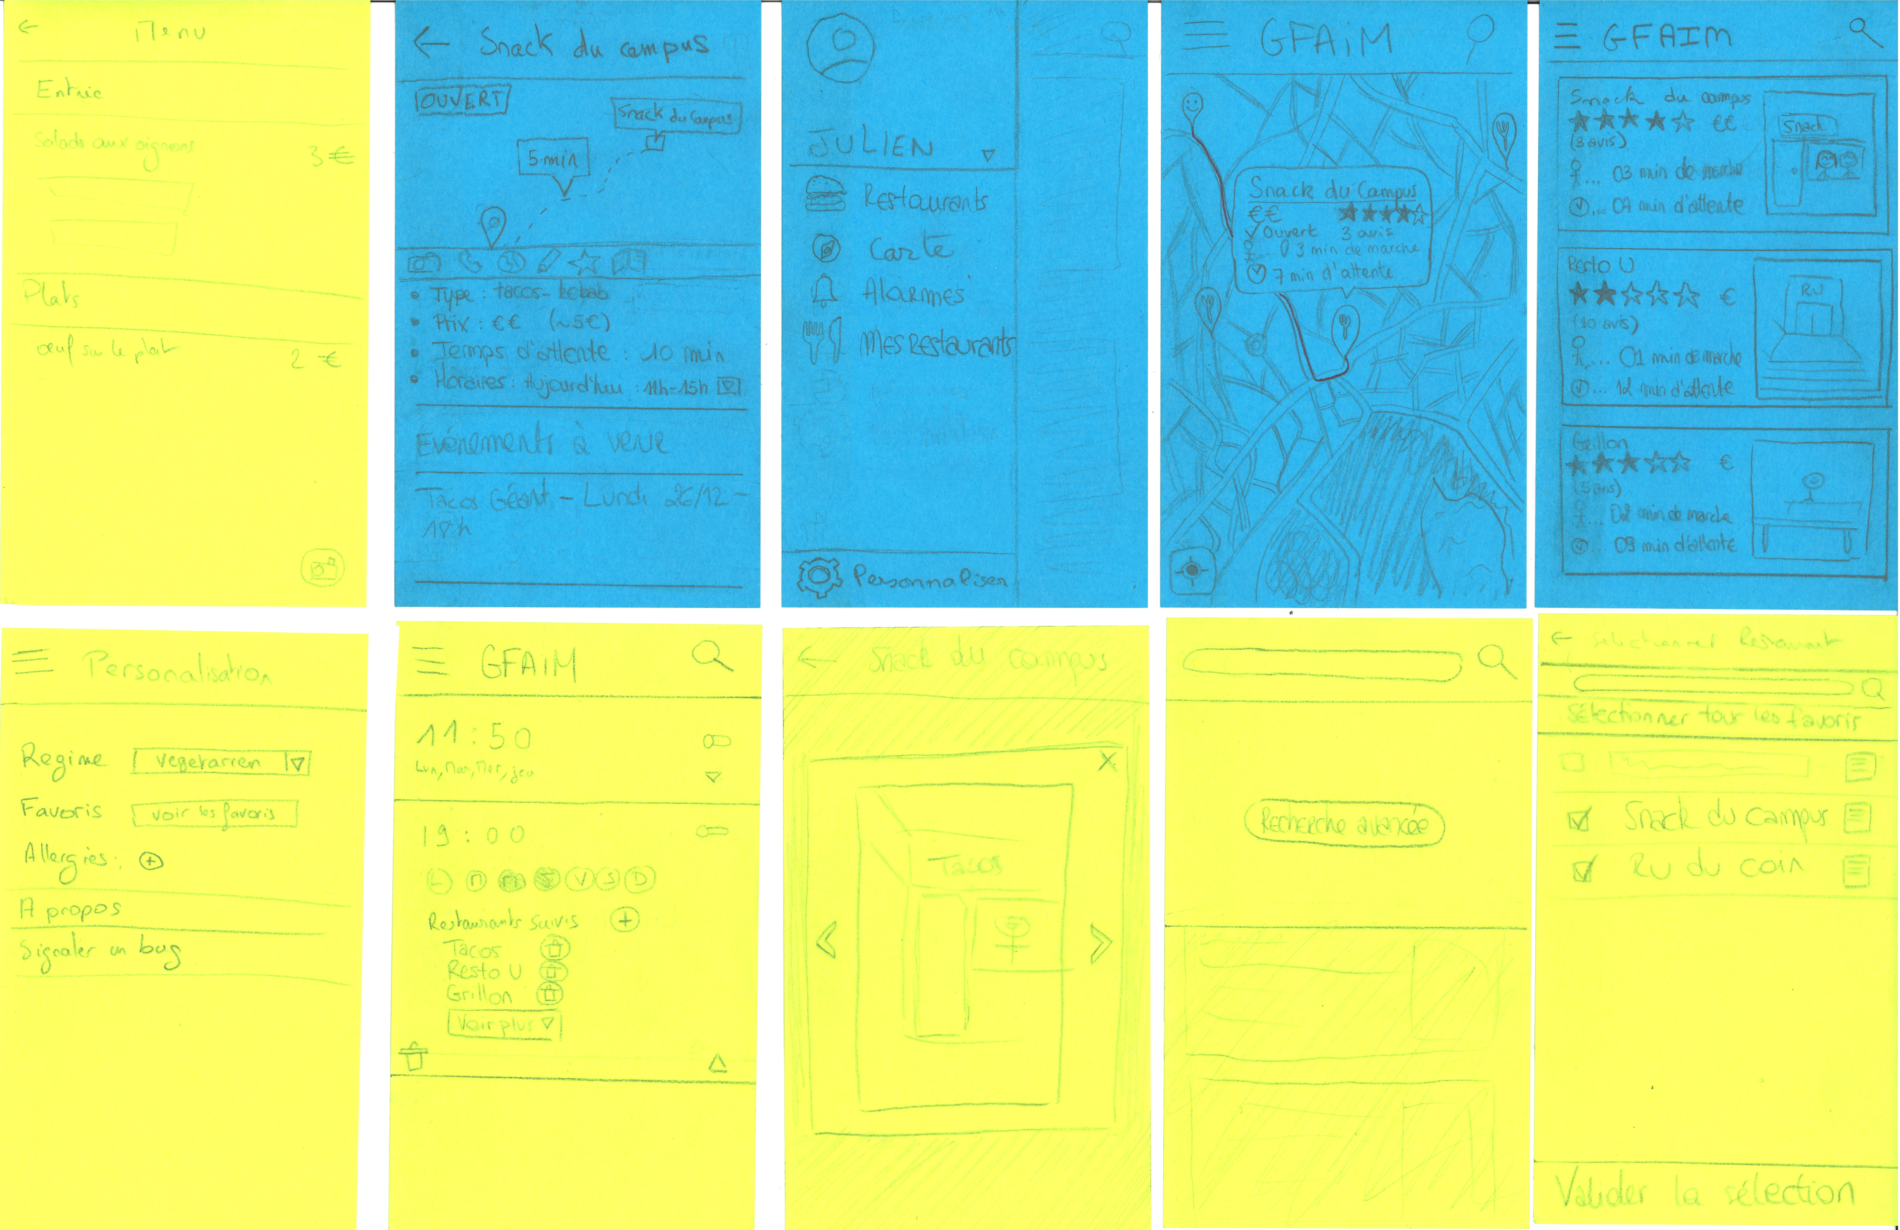
\includegraphics[width=15cm]{figures/mockups_1.png}}
    \noindent\makebox[\textwidth]{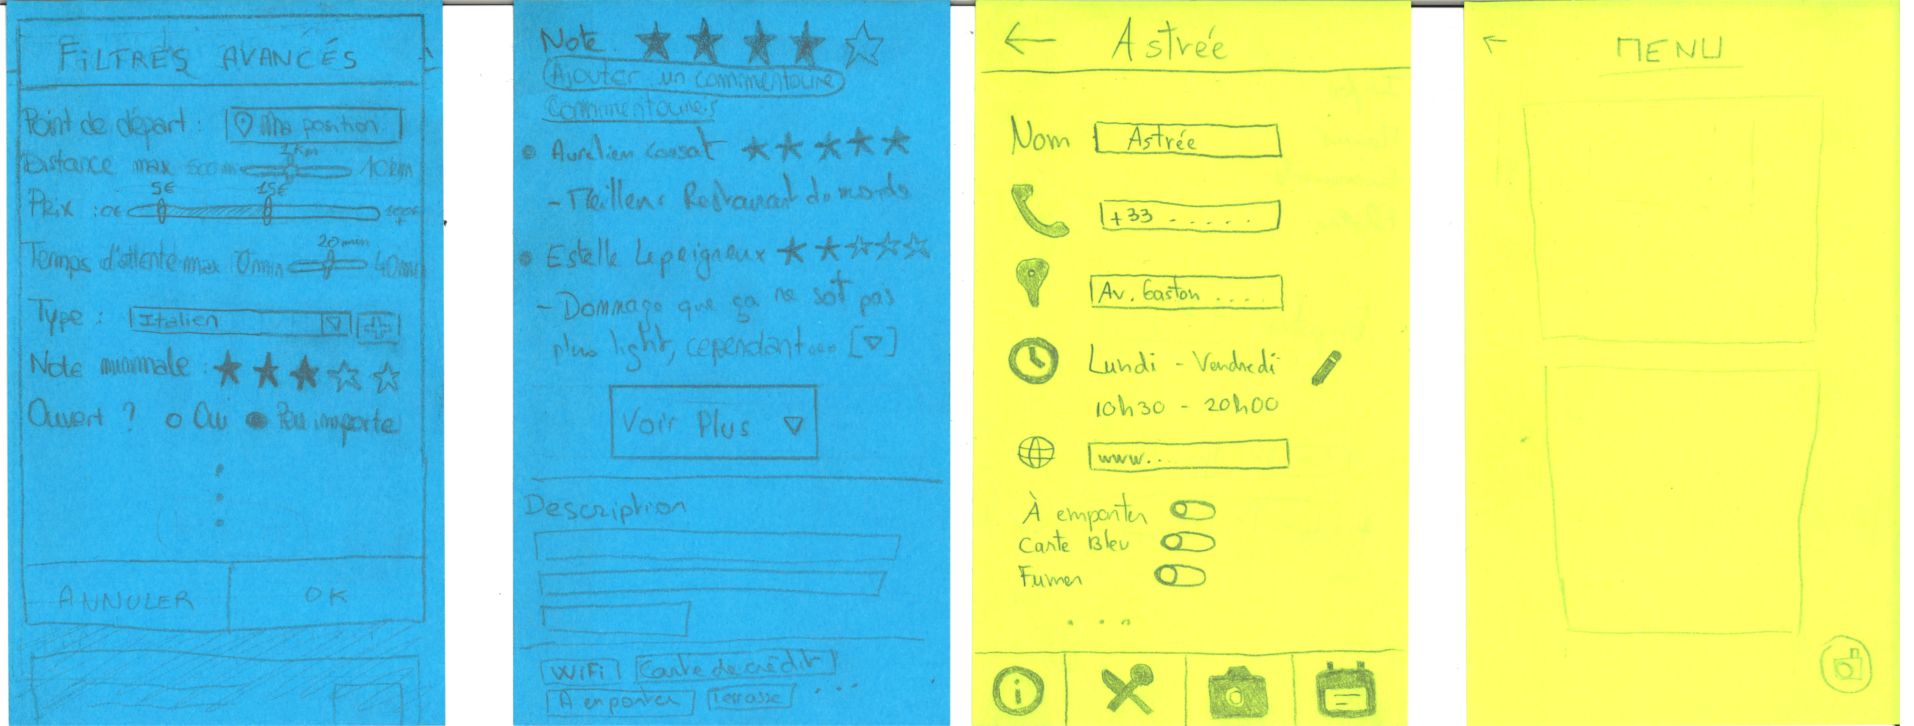
\includegraphics[width=15cm]{figures/mockups_2.png}}
    \caption{Mockups}
\end{figure}

Ces interfaces ont été réalisées sur des Post-It de la taille d'un écran de smartphone afin de nous placer dans les conditions réelles de taille et nous permettre de dimensionner les contrôles en connaissance de cause. Cela permet également de simuler l'usage en apposant le Post-It sur l'ecran d'un véritable smartphone pour simuler les clics avec nos doigts. Nous avons ainsi pu valider l'accessibilité des contrôles pour des utilisateurs présentant des morphologies différentes.

\part{Spécifications}
\setcounter{section}{0}
\section{Spécifications Minimales}

    Les spécifications données par le sujet sont les suivantes : \\
    
\begin{itemize}
    \item[\textbullet] Être disponible sur smartphone.
    \item[\textbullet] Suivre le guide de style d'Android et la charte graphique de l'INSA, dans la mesure du possible.
    \item[\textbullet] Prendre en compte différents types d'utilisateurs et différents types de points de restauration.
    \item[\textbullet] S'adapter aux différents types d'utilisateurs.
    \item[\textbullet] Fournir à l'utilisateur des informations pertinentes dans son contexte d'utilisation. \\
\end{itemize}

    Ces spécifications générales seront étendues dans par la suite. \\
    
    Les spécifications de notre application, concernant les deux premiers items de la liste ci dessus sont décrites dans le tableau ci-après. Elle décrive les différentes contraintes ergonomiques et d'accessibilité qui seront respectées par l'application développée. 

\begin{table}[H]
    \centering
    \caption{Tableau des spécifications minimales}
    \label{min-spec-table}
    \begin{tabular}{p{8cm}|p{8cm}}
        \bf{Spécification} & \bf{Justification} \\ \hline
        Chaque vue présentera une information spécifique & Ne pas diluer l'information importante dans une grande quantité d'informations inutiles \\ \hline
        Chaque vue présentera un nombre réduit de contrôles ($<= 10$) & \'Eviter d'introduire une complexité d'usage dans l'application \\ \hline
        Les contrôles seront regroupés dans les zones accessibles de l'écran &  Faciliter l'accès aux contrôles \\ \hline
        Les contrôles dont la fonctionnalité est la même (ex: suppression) sur des vues différentes partageront la même symbolique & Uniformiser, homogénéiser la symbolique de l'application \\ \hline
        Les contrôles et zones non utilisables seront grisées & Suggéger à l'utilisateur d'ignorer certaines zones ou contrôles et éviter les erreurs \\ \hline
        Les chaînes de caractères seront affichées avec une police adaptée au media utilisé & Permettre à l'utilisateur de ne pas se fatiguer \\ \hline
        Les polices de caractères et couleurs seront personnalisables dans le menu \og{}Personnalisation\fg{} & Permettre à l'utilisateur de paramétrer l'application selon ses besoins \\ \hline
        Les miniatures seront agrandies quand l'utilisateur clique dessus & Permettre à l'utilisateur de voir l'image quelque soit sa condition \\ \hline
        L'information principale sera présentée au centre de la vue & Faciliter l'accès à l'information en respectant les normes d'ergonomie \\ \hline
        Un bandeau présentant les contrôles globaux sera présent sur chaque vue & Donner accès aux contrôles depuis n'importe où dans l'application \\ \hline
        Un menu masquable sera présent sur la gauche de l'application et donnera accès aux principales fonctionnalités de l'application & Permettre à l'utilisateur de naviguer efficacement \\ \hline
        La profondeur de ce menu ne devra pas excéder deux niveaux & Conserver une interface simple et lisible pour l'utilisateur \\ \hline 
        Les messages d'erreur contiendront une description brève de l'erreur et la démarche à suivre pour la résoudre & Guider l'utilisateur de manière efficace en cas d'erreur \\ \hline
        Les notifications seront réglables pour laisser la liberté à l'utilisateur de les activer ou non & Ne pas imposer une fonctionnalité à l'utilisateur \\ \hline
        Les enchainements de vue de type processus seront limités à trois étapes si ils existent & Ne pas lasser l'utilisateur avec une procédure trop longue \\ \hline
        Les gestes et les inputs tactiles seront utilisés pour les barres de défilement qui n'apparaitront pas sur l'interface & Alléger l'interface graphique et améliorer l'expérience utilisateur en respectant les principes intuitifs \\
    \end{tabular}
\end{table}

    Le schéma ci-après décrit l'enchaînement des vues de l'application.
    
    \todo{Insérer le schéma d'enchainement des fenêtres ici}
\section{Spécifications Avancées}

\subsection{L'application prend en compte différents types d'utilisateurs}

Il y a deux profils principaux : le profil consommateur, qui inclue les étudiants du campus, les professeurs, les employés, etc., et le profil restaurateur, identique au profil consommateur à cela près qu'il peut administrer la page de son restaurant. \\
\bf{Fonctionnalités principales du profil consommateur :} accéder à la liste des restaurants à proximité et consulter leur détail (photos, menu, distance, temps d'attente, avis d'autres consommateurs\dots), voir les restaurants alentours sur une carte, régler des alarmes à une heure donnée pour le prévenir de l'état des indicateurs de certains restaurants. \\
\bf{Fonctionnalités principales du profil restaurateur :} les mêmes que celles du profil consommateur, avec une fonctionnalité principale supplémentaire : administrer la page de son propre restaurant.\\

\subsection{L'application prend en compte différents types de restaurants}

Lors de la recherche et de l'affichage de restaurants, il est possible de les trier selon leur type : restaurant, restaurant universitaire, restaurant-bar...

\subsection{L'application s'adapte aux différents types d'utilisateurs}

Consommateur : \\
\begin{table}[H]
    \centering
    \caption{Tableau des spécifications avancées du consommateur}
    \label{min-spec-table}
    \begin{tabular}{p{8cm}|p{8cm}}
 	\bf{Spécification} & \bf{Justification} \\ \hline
            Le consommateur peut accéder rapidement à tous les restaurants alentours grâce au menu, section \og{}Restaurants\fg{}. & L'intérêt principal de l'application pour le consommateur est de consulter les restaurants à proximité. \\ \hline
            Le consommateur peut rechercher un restaurant, soit directement avec son nom s'il le connaît, soit en indiquant des critères de recherche (temps d'attente, distance, etc.) pour une recherche avancée. & Cela permet au consommateur d'accéder rapidement à un/des restaurant(s) selon ce qu'il souhaite : obtenir l'état d'un restaurant précis, ou bien trouver un restaurant où il pourrait manger selon des critères qu'il aura définis. \\ \hline
            Le consommateur peut consulter les détails du restaurant, ce qui permet d'avoir une vue plus détaillée d'un restaurant choisi, notamment avec les avis d'autres utilisateurs et une mini-vue carte. & Ceci apporte un accès rapide aux indicateurs du restaurant, tout en gardant une vue compacte (certaines autres fonctionnalités étant accessible depuis cette vue). \\ \hline
            Depuis la vue détaillée du restaurant, le consommateur peut accéder à certaines autres fonctionnalités : photos du restaurant, téléphone, lien vers son site internet, laisser un avis, ajouter aux favoris, voir le menu. & Mettre toutes ces fonctionnalités directement dans la vue détaillée du restaurant aurait conduit à une page très remplie et peu lisible, d'où le choix de proposer d'y accéder seulement si le consommateur le souhaite. \\ \hline
            Le consommateur peut se repérer et voir les restaurants alentours à tout instant grâce au menu, section \og{}Carte\fg{}. & Le consommateur peut vouloir repérer un restaurant à proximité d'un endroit où il souhaite aller avant ou après manger. \\ \hline
            Le consommateur peut programmer une alarme pour être prévenu de l'état des indicateurs de certains restaurants, grâce à une notification, et donc sans avoir à ouvrir l'application. & La rapidité de l'accès à l'information est un critère primordial pour ce type d'application. \\
    \end{tabular}
\end{table}

Restaurateur : \\

\begin{table}[H]
    \centering
    \caption{Tableau des spécifications avancées du restaurateur}
    \label{min-spec-table}
    \begin{tabular}{p{8cm}|p{8cm}}
        \bf{Spécification} & \bf{Justification} \\ \hline
            Le restaurateur peut changer les informations générales de son restaurant : numéro de téléphone, adresse\dots & Il est utile que le consommateur soit informé rapidement de tels changements. \\ \hline
            Le restaurateur peut ajouter des photos de son propre restaurant. & Il est intéressant pour le consommateur de voir à quoi ressemble le restaurant pour s'en faire une idée. \\ \hline
            Le restaurateur peut ajouter le menu de son restaurant. & Le consommateur peut vouloir consulter ce qu'il y a à manger au restaurant sans avoir à y aller. \\ \hline
            Le restaurateur n'a pas besoin de renseigner le temps d'attente dans son restaurant : cela est fait en temps réel grâce à un système annexe. & Entrer les temps d'attente à la main manquerait évidemment de précision. \\
    \end{tabular}
\end{table}

\part{Documentation}
\setcounter{section}{0}
\section{Documentation}

L'application \appname~propose à ces utilisateurs la possibilité de découvrir les restaurants qui l'entourent sur son campus. Cette application est également destinée aux restaurateurs qui peuvent ainsi inscrire leur restaurant et donner des informations sur le menu du jour ou les offres promotionnelles ainsi que les évènements qu'ils organisent.

\subsection{Guide pour le consommateur}

Chacune des fonctionnalités, qui sont à votre disposition en tant qu'utilisateur, fera l'objet d'un paragraphe expliquant comment vous pouvez l'utiliser.

\todo{À completer : paragraphe explicatif pour chaque fonctionnalité}

\begin{itemize}
    \item[] \bf{Consultation des restaurants}
    \item[] \bf{Consultation les détails d'un restaurants}
    \item[] \bf{Recherche d'un restaurant}
    \item[] \bf{Trouver l'emplacement d'un restaurant}
    \item[] \bf{Paramétrage d'une alarme}
\end{itemize}

\subsection{Guide pour le restaurateur}

\todo{À completer}

\part{Bilan technique}
\setcounter{section}{0}
\todo{inclure ici le fichier du bilan technique}

\part{Suivi de projet}
\setcounter{section}{0}
\todo{inclure ici le fichier du suivi de projet}

\appendix
\todo{Ajouter l'anexe des résultats}

%%% End document
\end{document}
